\section{Research methodology}
The development process from Heath et al.~\cite{heath2009survey}, see figure~\ref{fig:steps_simulation},  has been followed.

The process consists of several rounds, its follows the agile or iterate management pattern.

\paragraph{Formulating the problem and objectives}

The formulation of the problem and objectives is complete; they are mentioned as the research goals in the previous section.

\paragraph{Conceptional validation}

The second round consists of building and validating the conceptual model.

%It relies upon known system theories, drives model development, and dictates the variety of assumptions required in any model abstraction process.

The importance of the conceptional model is mentioned by Heath et al.~\cite{heath2009survey}: the conceptual model forms the foundation of an ABM model; an invalid conceptual model indicates the model may not be an appropriate representation of reality.

Therefore, in this round, the abstraction level will be determined.

The model-based approach eliminates all variables not directly related to the problem and preserves only the essence of the situation.

The model must, in a highly abstract way, still mimic some actual behavior and real-world elements.

The conceptional model consists of:

\begin{itemize}
    \item Agents along with their behavior rules.
    \item A world with roads, buildings, and their rules.
\end{itemize}


All other interesting variables must be defined, such as the simulation period, the number of agents of each type, whether agents can leave, and when.

\paragraph{Translate into computer model}

This round converts the conceptual model into computer code.

As mentioned, this study's multi-agent programmable modeling environment was NetLogo~\footnote{\url{ccl.northwestern.edu/netlogo/}}.

This environment and programming language needed some studying; for this, the NetLogo online user manuals~\footnote{\url{ccl.northwestern.edu/netlogo/docs/}} and other existing models were used.

Understanding the temporal programming model is key.

In essence in each tick (the smallest time unit in NetLogo) all behavior rules must be evaluated.

A large part of the world is based on an existing model,i.e., the Taxi Cab model~\cite{dongpingtaxicabs2019} see figure~\ref{fig:taxicabmodel}.


\begin{figure}
    \centering

    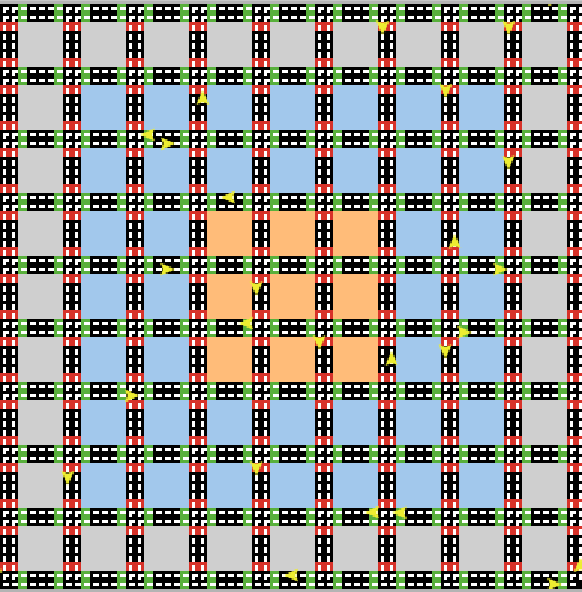
\includegraphics[width=8cm]{sections/pics/Taxi Cabs}

    \caption{Taxi Cab Model}

    \label{fig:taxicabmodel}

\end{figure}



\paragraph{Run simulations and obtain results}
With the model in place, the simulations can be run.
To get certain results the model still is subjected to change in this step.

A Python package called pyNetLogo~\footnote{\url{pynetlogo.readthedocs.io/}} was used to automate the simulation and set some variables.
This package has the ability to start a NetLogo program, set some variables, and run it for some time (ticks).
It enables the running of many simulations and save the results.

First task is finding a stable situation where after some time no agents leave.
This is a baseline.

After this, using the baseline settings, simulations will be run where deliverers may leave.
Then compare the outcomes.
















